\documentclass[]{article}
\usepackage[T1]{fontenc}
\usepackage{lmodern}
\usepackage{amssymb,amsmath}
\usepackage{ifxetex,ifluatex}
\usepackage{fixltx2e} % provides \textsubscript
% use upquote if available, for straight quotes in verbatim environments
\IfFileExists{upquote.sty}{\usepackage{upquote}}{}
\ifnum 0\ifxetex 1\fi\ifluatex 1\fi=0 % if pdftex
  \usepackage[utf8]{inputenc}
\else % if luatex or xelatex
  \ifxetex
    \usepackage{mathspec}
    \usepackage{xltxtra,xunicode}
  \else
    \usepackage{fontspec}
  \fi
  \defaultfontfeatures{Mapping=tex-text,Scale=MatchLowercase}
  \newcommand{\euro}{€}
\fi
% use microtype if available
\IfFileExists{microtype.sty}{\usepackage{microtype}}{}
\usepackage[margin=1in]{geometry}
\usepackage{color}
\usepackage{fancyvrb}
\newcommand{\VerbBar}{|}
\newcommand{\VERB}{\Verb[commandchars=\\\{\}]}
\DefineVerbatimEnvironment{Highlighting}{Verbatim}{commandchars=\\\{\}}
% Add ',fontsize=\small' for more characters per line
\usepackage{framed}
\definecolor{shadecolor}{RGB}{248,248,248}
\newenvironment{Shaded}{\begin{snugshade}}{\end{snugshade}}
\newcommand{\KeywordTok}[1]{\textcolor[rgb]{0.13,0.29,0.53}{\textbf{{#1}}}}
\newcommand{\DataTypeTok}[1]{\textcolor[rgb]{0.13,0.29,0.53}{{#1}}}
\newcommand{\DecValTok}[1]{\textcolor[rgb]{0.00,0.00,0.81}{{#1}}}
\newcommand{\BaseNTok}[1]{\textcolor[rgb]{0.00,0.00,0.81}{{#1}}}
\newcommand{\FloatTok}[1]{\textcolor[rgb]{0.00,0.00,0.81}{{#1}}}
\newcommand{\CharTok}[1]{\textcolor[rgb]{0.31,0.60,0.02}{{#1}}}
\newcommand{\StringTok}[1]{\textcolor[rgb]{0.31,0.60,0.02}{{#1}}}
\newcommand{\CommentTok}[1]{\textcolor[rgb]{0.56,0.35,0.01}{\textit{{#1}}}}
\newcommand{\OtherTok}[1]{\textcolor[rgb]{0.56,0.35,0.01}{{#1}}}
\newcommand{\AlertTok}[1]{\textcolor[rgb]{0.94,0.16,0.16}{{#1}}}
\newcommand{\FunctionTok}[1]{\textcolor[rgb]{0.00,0.00,0.00}{{#1}}}
\newcommand{\RegionMarkerTok}[1]{{#1}}
\newcommand{\ErrorTok}[1]{\textbf{{#1}}}
\newcommand{\NormalTok}[1]{{#1}}
\usepackage{graphicx}
% Redefine \includegraphics so that, unless explicit options are
% given, the image width will not exceed the width of the page.
% Images get their normal width if they fit onto the page, but
% are scaled down if they would overflow the margins.
\makeatletter
\def\ScaleIfNeeded{%
  \ifdim\Gin@nat@width>\linewidth
    \linewidth
  \else
    \Gin@nat@width
  \fi
}
\makeatother
\let\Oldincludegraphics\includegraphics
{%
 \catcode`\@=11\relax%
 \gdef\includegraphics{\@ifnextchar[{\Oldincludegraphics}{\Oldincludegraphics[width=\ScaleIfNeeded]}}%
}%
\ifxetex
  \usepackage[setpagesize=false, % page size defined by xetex
              unicode=false, % unicode breaks when used with xetex
              xetex]{hyperref}
\else
  \usepackage[unicode=true]{hyperref}
\fi
\hypersetup{breaklinks=true,
            bookmarks=true,
            pdfauthor={Nikolai Gorte \& Simon Schoemaker},
            pdftitle={Using EnviroCar data in R},
            colorlinks=true,
            citecolor=blue,
            urlcolor=blue,
            linkcolor=magenta,
            pdfborder={0 0 0}}
\urlstyle{same}  % don't use monospace font for urls
\setlength{\parindent}{0pt}
\setlength{\parskip}{6pt plus 2pt minus 1pt}
\setlength{\emergencystretch}{3em}  % prevent overfull lines
\setcounter{secnumdepth}{0}

%%% Change title format to be more compact
\usepackage{titling}
\setlength{\droptitle}{-2em}
  \title{Using EnviroCar data in R}
  \pretitle{\vspace{\droptitle}\centering\huge}
  \posttitle{\par}
  \author{Nikolai Gorte \& Simon Schoemaker}
  \preauthor{\centering\large\emph}
  \postauthor{\par}
  \predate{\centering\large\emph}
  \postdate{\par}
  \date{November 20, 2014}




\begin{document}

\maketitle


\section{enviroCaR - Analysis of Car
Trajectories}\label{envirocar---analysis-of-car-trajectories}

The capital R in the name ``enviroCaR'' obviously reveals that it is the
R package corresponding to the project we will work on
(\url{https://envirocar.org/}). In general, enviroCaR provides basic
functions to load and analyse measurements from the enviroCar server
(Pebesma, Stasch, and Wirwahn 2014).

R is a open-source software for general data analysis. It compiles and
runs on a wide variety of platforms and provides a big sample of
statistical and graphical methods. Furthermore, R is easily extendable
through a massive amount of so-called packages. Currently, there are
round about 6000 packages available on the ``Comprehensive R Archive
Network'', short called CRAN. The number of developers and published
packages are growing continuously. Additionally, each package has got
help pages, several documentations and useful example code chunks (R
Core Team 2014).

As mentioned before R packages are usually available on CRAN and can be
installed from there relatively straightforward. However, the EnviroCaR
package is not on CRAN as yet and needs to be installed from github
(\url{https://github.com/enviroCar/enviroCaR}). For the installation you
can use Hadley`s devtools package to accomplish this easily (Wickham and
Chang 2014).

\begin{Shaded}
\begin{Highlighting}[]
\KeywordTok{library}\NormalTok{(devtools)}
\KeywordTok{install_github}\NormalTok{(}\StringTok{'enviroCaR'}\NormalTok{, }\StringTok{'enviroCar'}\NormalTok{)}
\end{Highlighting}
\end{Shaded}

\begin{itemize}
\itemsep1pt\parskip0pt\parsep0pt
\item
  Trajectories
\item
  Track
\item
  Tracks
\item
  TracksCollection
\item
  EnviroCaR (github)
\item
  ImportSingleTrack
\item
  ImportEnviroCar
\end{itemize}

\newpage

\section{Aggregation}\label{aggregation}

One function provided by the enviroCaR package is
\texttt{aggregateTrack}. This function is used to aggregate measurements
of a Track object.\\It is possible to specify the phenomenon for
aggregation, the interval size of measurements that have to be
aggregated and a function for aggregation (e.g.~mean).\\Aggregation over
time is not possible at the moment! In Figure 1 we can see an example of
an aggregated track. The raw track (black) is aggregated to six points
(red).

\begin{figure}[htbp]
\centering
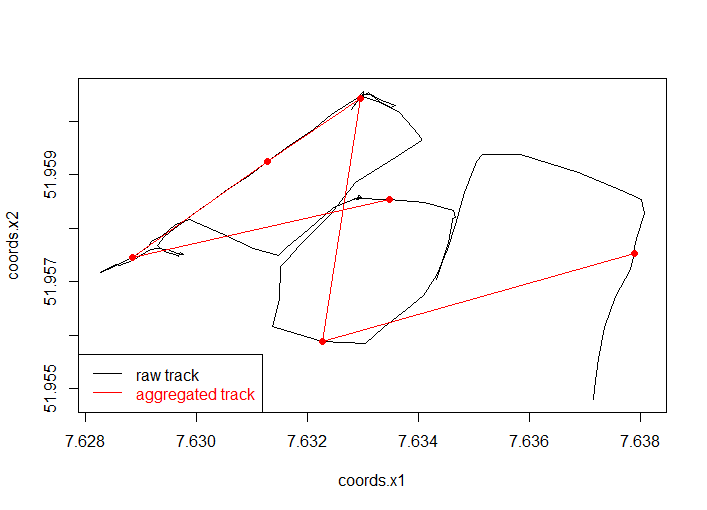
\includegraphics{figures/agg.png}
\caption{Aggregated Track}
\end{figure}

\section{Map Matching}\label{map-matching}

Map matching is the process of matching GPS trajectories to a digital
road network and is done using map matching algorithms. This is
necessary because positions acquired from GPS, as they are in the
enviroCaR project, are affected by several kind of errors resulting in
inaccurate positions on maps.\\Matching the enviroCar trajectories to a
digital road network would not only improve the visual representation,
but could also be useful when it comes to analysis or comparison of
trajectories.

One possible way of achieving this is the \texttt{fuzzyMM} package
(Gorte 2014) which implements a fuzzy logic based map matching
algorithm.\\As can be seen in Figure 2 the raw GPS positions are matched
to road segments after the application of the map matching algorithm.

\begin{figure}[h!]
  \centering
    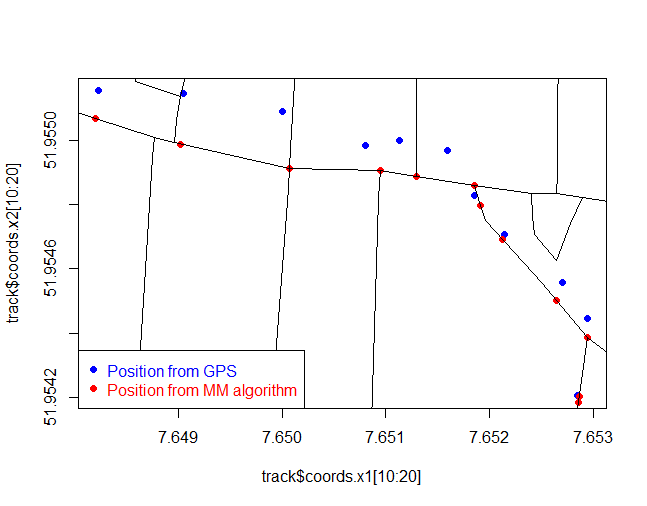
\includegraphics[width=1\textwidth]{figures/urban.png}
    \caption{Map Matching}
    \label{fig:mm}
\end{figure}

At the moment fuzzyMM only works for \texttt{SpatialPointsDataFrame}
objects which contain the GPS positions of the track and GPS data such
as HDOP, speed and bearing. Since all of this is also included in the
\texttt{Track} class, it should be no problem to modify the function to
work with the trajectory classes.

\section{Conclusion}\label{conclusion}

As can be seen in the previous sections, what we can do with the
enviroCar data in R until now is mostly basics. We can load enviroCar
tracks into R, where they are represented by the classes from the
trajectories package and we can also do some basic plotting and
aggregate measurements of a Track object.

So there are several things that could be done in the future and maybe
in the scope of this course. This, for example, includes implementing
map matching to assign trajectories to road segments. Other things to
think about are aggregation methods, e.g.~the aggregation over multiple
trajectories or aggregation over space and/or time. What may be also
important and interesting is comparing trajectories of one driver and
also comparing trajectories between different drivers.

\section*{References}\label{references}
\addcontentsline{toc}{section}{References}

Gorte, Nikolai. 2014. \emph{fuzzyMM: Map Matching Using Fuzzy Logic}.
\url{http://CRAN.R-project.org/package=fuzzyMM}.

Pebesma, Edzer, Christoph Stasch, and Jan Wirwahn. 2014.
\emph{enviroCaR: Analysis of Car Trajectories Provided by EnviroCar
Project}. \url{https://github.com/enviroCar/enviroCaR}.

R Core Team. 2014. \emph{R: A Language and Environment for Statistical
Computing}. Vienna, Austria: R Foundation for Statistical Computing.
\url{http://www.R-project.org/}.

Wickham, Hadley, and Winston Chang. 2014. \emph{devtools: Tools to Make
Developing R Code Easier}.
\url{http://CRAN.R-project.org/package=devtools}.

\end{document}
